% !TEX root = /Users/parth/active_projects/rnn-memorization/11-20-23/update.tex
\input{/Users/parth/Documents/_header.tex}

\title{update on rnn memorization}
\date{\vspace{-1em}Monday, November 20, 2023\vspace{1em}}
\author{}

\DeclareMathOperator{\argmax}{argmax}

\begin{document}
\maketitle

RNNs are capable of memorizing strings — if you repeatedly train the model on a string, it'll eventually overfit and only output that string. The mechanism for systematic memorization of strings is not well understood. This line of work seeks to understand that phenomenon.

We can use a simplified neural network architecture to study this. As it turns out, memorization can be done without any nonlinearity. Choose an alphabet $\Sigma$ and let $n = |\Sigma|$. We fix matrices $W_h, W_x, W_y$ and a bias vector $b_y$ and define the following update rule:
\begin{align*}
    h_i &= W_h h_{i-1} + W_x x_i \\
    y_i &= W_y h_i + b_y \\
    x_{i + 1}[j] &= \begin{cases}
        1 & \text{if } j = \argmax_k y_i[k] \\
        0 & \text{otherwise}
    \end{cases}
\end{align*}
Here, the input and output $x_i$ and $y_i$ are vectors of length $n$ and the hidden state $h_i$ is a vector of length $d$ (not necessarily equal to $n$). The input $x_i$ is a one-hot vector, and the output $y_i$ is a vector of logits. This definition differs from the standard RNN in a few ways: we eliminate the nonlinearity on $h_i$ and $y_i$, we don't add a bias vector to $h_i$, and we don't apply softmax to $y_i$. Small modifications of our approach allow it to work for the standard RNN model, but we don't need all that complexity.

Typically, the hidden state starts at the origin, $h_0 = 0$, and the RNN reads a \verb|<START>| token which moves the hidden state to the initial nonzero position. By generality, we leave \verb|<START>| out of the alphabet $\Sigma$ and assume that we can choose the initial hidden state $h_0$. We will return to the question of how to terminate the string with an \verb|<END>| token later.

\section*{${(0^a 1^b)}^+$}
Suppose the alphabet only has two characters, $\Sigma = \{0, 1\}$. We represent $0$ as the first column of the identity, $(1, 0)$, and $1$ as the next, $(0, 1)$. We can memorize the string ${(0^a 1^b)}^+$ with $d = 2$. 

This solution completely ignores the input $x_i$, taking $W_x = 0$. Let $W_h$ be the counterclockwise rotation by $\theta = \f{2\pi}{a + b}$. Then, taking $h_0$ on the unit circle, it will walk around the circle $a + b$ times before returning, tracing out a polygon, as seen in Figure~\ref{fig:octagon}.

\begin{figure}[h]
\centering
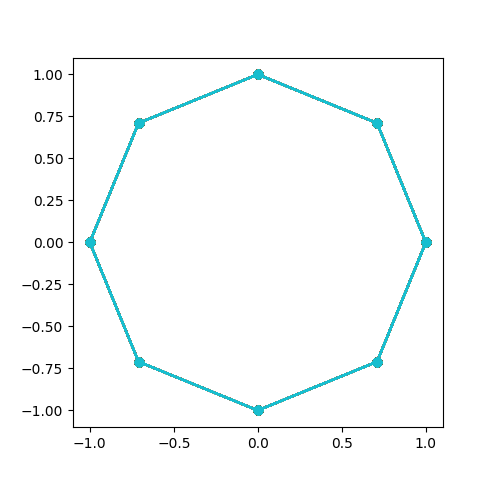
\includegraphics[width=7cm]{img/octagon.png}
\caption{The hidden state $h_i$ traces out an octagon when $a + b = 8$.}\label{fig:octagon}
\end{figure}

Then, we can pick any hyperplane and origin point on the hyperplane and compute $W_y$ and $b_y$ so that hidden states to the right of the hyperplane get mapped to $0$ and hidden states to the left get mapped to $1$. This is possible because the hidden states are bounded, so we can shift them into the upper-right quadrant and then rotate the picture so the hyperplane is the line $y = x$.

\begin{figure}[h]
\centering
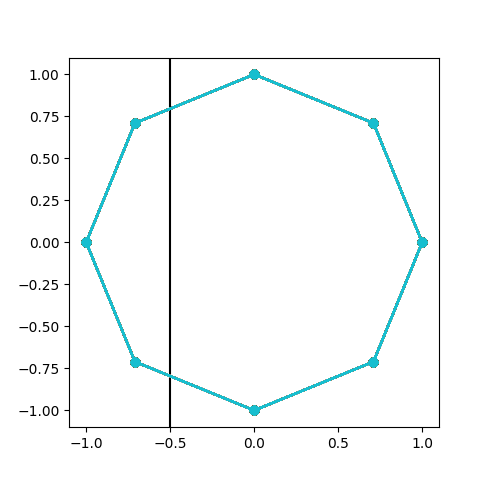
\includegraphics[width=7cm]{img/octagon-with-hyperplane.png}
\caption{Choosing $W_y$ and $b_y$ corresponding to the black line above will output $(0^5 1^3)^+$.}\label{fig:octagon-with-hyperplane}
\end{figure}

This shows how an RNN can memorize ${(0^a 1^b)}^+$ with $d = 2$.

\section*{${(\sigma_1^{a_1} \sigma_2^{a_2} \cdots \sigma_k^{a_k})}^+$}
The expression ${(\sigma_1^{a_1} \sigma_2^{a_2} \cdots \sigma_k^{a_k})}^+$ represents any periodic string. If we have an \verb|<END>| token we can  choose $\sigma_k = \verb|<END>|$ and $a_k = 1$ to make the string finite. We will now present a solution for this problem with $d = \sum_{j = 1}^k a_j$. By abuse of notation, we'll let $\sigma_j$ be the $j$th column of the $n \times n$ identity matrix, so $\sigma_j$ is a one-hot vector (rather than a symbol corresponding to that vector). Once again, we ignore the input $x_i$ and take $W_x = 0$.

Consider the representation of the symmetric group $S_d \to GL_d$ acting on the hidden space $\R^d$ as \[ \sigma \cdot \bpmx v_1 \\ \vdots \\ v_d \epmx = \bpmx v_{\sigma(1)} \\ \vdots \\ v_{\sigma(d)} \epmx. \] Then take $c$ to be the cyclic permutation $(1 \; 2 \; \cdots \; d)$ and let $W_h$ be the representation of $c$. 

Let $h_1$ be the first column of the $d \times d$ identity matrix. Then $h_2$ is the second column of the identity matrix, and so on. The hidden states repeat after $d$ steps with $h_{d + 1} = h_1$. This means we can take \[ W_y = \bbmx
    \;\vline &  & \vline & \vline &  & \vline &  & \vline &  & \vline\; \\
    \;\sigma_1 & \cdots & \sigma_1 & \sigma_2 & \cdots & \sigma_2 & \cdots & \sigma_k & \cdots & \sigma_k\; \\
    \;\vline &  & \vline & \vline &  & \vline &  & \vline &  & \vline\; \\
\ebmx. \] In words, this is the $n \times d$ matrix which has $a_j$ copies of $\sigma_j$ in the $j$th block. Since $h_l$ is a one-hot vector, $W_y h_l$ is the $l$th column of of $W_y$, and we've designed this matrix so $W_y h_l$ is the desired vector $\sigma_j$.

This shows how an RNN can memorize any string with period $d$ using a hidden state of dimension $d$.

\brk We chose $c = (1 \; 2 \; \cdots \; d)$, but there are many valid choices for $c$. In fact, for any $1 \leq j < d$, where $j$ is coprime with $d$, we can choose $W_h$ to be the representation of $c^j$. There are $\varphi(n)$ such elements where $\varphi$ is Euler's totient function. In particular $\varphi(n) \geq \sqrt{n/2}$. The existence of other valid weights $W_h$ might suggest some ``inefficiency'' in the size of $d$, which we'll explore next. \erk

\section*{How small can we make $d$?}
In the previous section, we used a hidden state of dimension $d = \sum_{j = 1}^k a_j$. We've seen that, under some circumstances, we can do better. In the first section we were able to represent $(\sigma_1^{a_1} \sigma_2^{a_2})^+$ with $d = 2$, regardless of $a_1$ and $a_2$. Under some assumptions, we can show that $d = 2$ is optimal.

Assume that, as is the case with the two solutions we constructed, $W_x = 0$. Let $p = \sum_{j = 1}^k a_j$ be the period of the string and assume that $W_h^p = \I$, as is the case with our constructions. We have a complete solution where the hidden dimension $d = p$ — we'll focus on trying to make $d < p$.

To build the theory about $W_h$, we'll use the following definitions and facts.

\bddefn[Minimal polynomial] The minimal polynomial of a $d \times d$ matrix $A$ is the monic polynomial $m_A(x)$ of least degree such that $m_A(A) = 0$.\eddefn

\bddefn[Characteristic polynomial] The characteristic polynomial of a $d \times d$ matrix $A$ is $\chi_A(x) = \det(xI - A)$. The degree of $\chi_A$ is $d$.\eddefn

\bddefn[Order] The order of a $d \times d$ matrix $A$ is $\ord(A) = \min \{p : A^p = \I\}$.\eddefn

\bllem If $p(x)$ is a polynomial with $p(A) = 0$, then the minimal polynomial of $A$ divides $p$, denoted $m_A \divides p$.\ellem

\bpf Since $\deg m_A \leq \deg p$, we can use the division algorithm to write $p(x) = q(x) m_A(x) + r(x)$ where $\deg r < \deg m_A$. Then $0 = p(A) = q(A) m_A(A) + r(A) = r(A)$, so the matrix $A$ annihilates $r$. By the minimality of $\deg(m_A)$ we conclude that $r(x) = 0$, so $p(x) = q(x) m_A(x)$ or, in short, $m_A \divides p$.\epf

Now, since $W_h^p = \I$, the matrix $W_h$ annihilates the polynomial $q(x) = x^p - 1$. By the Lemma, the minimal polynomial of $W_h$ divides $q(x)$. Next, we can factor $q$ to see what our options are for the minimal polynomial.

The polynomial $q$ splits over $\C$, where we can write \[ q(x) = \prod_{j=1}^p \left(x - e^{2 \pi i \frac{j}{p}}\right). \] Indeed, the $1 \times 1$ matrix $W_h = e^{2 \pi i / p}$ satisfies $W_h^p = \I$. For a moment, let's look at how it factors over $\Q$: \[ q(x) = \prod_{j \divides p} \Phi_j(x), \] where $\Phi_j$ is the $j$th cyclotomic polynomial, i.e., \[ \Phi_j(x) = \prod_{\substack{1 \leq k \leq j \\ \gcd(k, j) = 1}} \left(x - e^{2 \pi i \frac{k}{j}}\right). \] The cyclotomic polynomials are irreducible over $\Q$, and have coefficients in $\{-1, 0, 1\}$.

This is a powerful decomposition. It allows us, for example, to prove that there are no $3 \times 3$ rational matrices with order $8$. To see this, suppose that $A$ is a $3 \times 3$ matrix with $A^8 = \I$. Then, the minimal polynomial $m_A$ divides $x^8 - 1$, which splits over $\Q$ as $x^8 - 1 = (x^4 + 1)(x^2 + 1)(x + 1)(x - 1)$. Since the characteristic polynomial $\chi_A$ has degree $3$, the degree $\deg m_A \leq 3$. This means that we need to build $m_A$ from the factors of $x^8 - 1$ with degree at most $3$, so $m_A \divides (x^2 + 1)(x + 1)(x - 1) = x^4 - 1$. Therefore, $A$ annihilates the polynomial $x^4 - 1$ so $A^4 = \I$ and $\ord(A) \leq 4$.

If we were restricted to rational matrices, we could use this theory to find which hidden dimensions permit memorization of strings with period $p$. Over $\R$, we can combine \[ \left(x - e^{2 \pi i \f{j}{p}}\right)\left(x - e^{2 \pi i \f{p - j}{p}}\right) = x^2 - 2 \cos\left(2 \pi \f{j}{p}\right) x + 1, \] and by repeatedly applying this identity we can write $q(x)$ as a product of quadratic polynomials. This shows that, in general, the best hidden dimension we can hope for is $d = 2$ where the rotation matrices have order $p$.

\end{document}